\documentclass[review,3p]{elsarticle}
\usepackage{lmodern}
\usepackage{amsmath,amssymb,amsfonts}
\usepackage{graphicx,textcomp,xcolor,booktabs,url,hyperref,balance}

\usepackage{lineno}

\journal{Applied Soft Computing}

\begin{document}
\title{One Model, Three Tasks: Multi-Task Fine-Tuning Provides Implicit Regularization Against Label Hallucination in SOC Classification}
\author[kmitl]{Nutthakorn Chalaemwongwan\corref{cor1}}
\cortext[cor1]{Corresponding author}
\ead{nutthakorn.ch@kmitl.ac.th}
\address[kmitl]{Department of Computer Engineering, KOSEN-KMITL, King Mongkut's Institute of Technology Ladkrabang, Bangkok, Thailand}
\begin{frontmatter}

\begin{highlights}
\item Multi-task format provides implicit regularization for label compliance (+5.7\% F1).
\item Single model handles classification, triage, and severity assessment simultaneously.
\item Format regularization prevents label hallucination without additional training data.
\item Joint training creates shared representations that improve compliance.
\item Practical deployment: one model replaces three task-specific classifiers.
\end{highlights}

\begin{abstract}
SOC alert processing requires simultaneous classification, triage, and attack category identification---tasks traditionally handled by separate models or sequential pipelines. We compare multi-task fine-tuning (one model, all dimensions in a single pass) against single-task specialists on Qwen3.5-0.8B using QLoRA across 3 random seeds. Multi-task models match single-task performance on low-entropy dimensions (Classification $H=0.083$, Triage $H=0.834$) and provide \textbf{implicit regularization} on the challenging Attack Category dimension ($H=1.24$): multi-task mean strict F1 = $0.886 \pm 0.053$ vs.\ single-task = $0.829 \pm 0.052$ across 3 seeds. At the most divergent seed (999), multi-task produces 33 errors vs.\ single-task's 1,107---a \textbf{33$\times$ reduction}. We identify \emph{format learning} as the mechanism: the structured output schema $\langle$field: value $|$ field: value$\rangle$ constrains vocabulary selection, suppressing pre-training knowledge bleed-through. We formalize this as Format Regularization (Definition~1) and show it reduces hallucinated label vocabulary by $1.39\times$ on average. Multi-task deployment halves infrastructure complexity (1~model vs.\ 3) and reduces latency (1~inference pass vs.\ 3), with no accuracy penalty on easy tasks and a consistent advantage on hard tasks.
\end{abstract}

\begin{keyword}
multi-task learning \sep SOC classification \sep seed sensitivity \sep label compliance \sep implicit regularization \sep format learning
\end{keyword}

\end{frontmatter}

%% ===== INTRODUCTION =====
\section{Introduction}

SOC alert processing is inherently multi-dimensional: each alert requires a binary classification (Malicious vs.\ Benign), a triage decision (Escalate/Investigate/Monitor), an attack category label (8 classes from MITRE ATT\&CK), and a priority score (0--1). Two deployment strategies exist:

\begin{enumerate}
\item \textbf{Single-task (ST)}: 3 separate models, each optimized for one dimension. Requires 3 inference passes and 3$\times$ deployment infrastructure.
\item \textbf{Multi-task (MT)}: 1 model generating all dimensions in a single structured output. Requires 1 inference pass.
\end{enumerate}

The conventional concern with multi-task learning is \emph{negative transfer}---interference between tasks degrading performance on individual dimensions~\cite{zhang2022,standley2020}. Multi-task NLP research has produced mixed results: Caruana~\cite{caruana1997} demonstrated shared representations improve generalization, but subsequent work~\cite{standley2020} showed task grouping matters critically.

We find the opposite of negative transfer: multi-task training provides \emph{positive transfer} via implicit regularization, improving label compliance on the hardest dimension (Attack Category, $H=1.24$ bits). This improvement is not from better feature learning---both MT and ST achieve identical performance on easy dimensions---but from \emph{format learning}: the structured output schema constrains vocabulary selection.

This finding has direct deployment implications: MT is strictly superior to ST for SOC classification, providing equal or better accuracy with half the infrastructure and one-third the latency.

Our contributions:
\begin{enumerate}
\item We demonstrate that MT matches ST on easy dimensions ($H < 1$ bit) and \emph{outperforms} on hard dimensions (+5.7 points on $H = 1.24$).
\item We identify \emph{format learning} as the mechanism: structured $\langle$field: value$\rangle$ output constrains vocabulary, reducing hallucination by $1.39\times$ on average and up to $33\times$ at specific seeds.
\item We quantify seed sensitivity differences between MT and ST: both exhibit high variance on Attack Category ($\text{std} \approx 0.05$), but MT has consistently higher mean.
\item We formalize Format Regularization (Definition~1) and provide evidence for its mechanism.
\item We provide deployment recommendations showing MT dominates on all operational dimensions: fewer models, fewer passes, higher F1.
\end{enumerate}

Our companion studies established the label hallucination phenomenon~\cite{p3}, its scaling behavior~\cite{p6}, cost implications~\cite{p7}, rank sensitivity~\cite{p22}, architecture effects~\cite{p21}, cascade routing~\cite{p5}, and entropy-based classifier selection~\cite{p8}. This paper identifies a \emph{training-time} mitigation via multi-task format constraints.

The remainder of this paper is organized as follows: Section~II reviews multi-task learning and negative transfer. Section~III describes the experimental setup. Section~IV compares MT and ST across 3 seeds with error analysis. Section~V discusses the format learning mechanism, deployment comparison, and limitations. Section~VI concludes with guidelines.

%% ===== RELATED WORK =====
\section{Related Work}

\subsection{Multi-Task Learning}
Caruana~\cite{caruana1997} established that multi-task learning improves generalization through shared representations, acting as inductive bias. T5~\cite{raffel2020} demonstrated casting all NLP tasks as text-to-text problems, achieving state-of-the-art results across diverse benchmarks with a single model. FLAN~\cite{wei2022} extended this to instruction tuning, showing that training on diverse task formats improves zero-shot generalization. Liu et~al.~\cite{liu2019} proposed MT-DNN, combining multi-task learning with pre-trained representations for NLU tasks.

\subsection{Negative Transfer}
Negative transfer occurs when jointly training on dissimilar tasks degrades individual task performance~\cite{zhang2022}. Standley et~al.~\cite{standley2020} showed that task grouping strategy critically affects transfer quality: tasks with similar gradients benefit from sharing, while conflicting gradients cause interference. Yu et~al.~\cite{yu2020} proposed gradient surgery (PCGrad) to mitigate conflicts between task gradients. Our tasks share a common input (network alert features) with different output distributions: Classification is trivial ($H = 0.083$), Triage is easy ($H = 0.834$), and Attack Category is challenging ($H = 1.24$). The risk of negative transfer is highest for Attack Category.

\subsection{Multi-Task in Cybersecurity}
SOC environments naturally present multi-task scenarios: classification, severity assessment, threat categorization, and response recommendations. Ferrag et~al.~\cite{ferrag2024} surveyed LLM applications in cybersecurity but treated tasks independently. The UNSW-NB15 dataset~\cite{moustafa2016} and its derivative SALAD provide the multi-dimensional label structure necessary for multi-task evaluation. Ji et~al.~\cite{ji2023} documented hallucination in NLG; Gekhman et~al.~\cite{gekhman2024} showed fine-tuning increases hallucination. LoRA~\cite{hu2022} and QLoRA~\cite{dettmers2023} enable efficient fine-tuning on consumer hardware. Kapoor and Narayanan~\cite{kapoor2023} emphasized data integrity, motivating our use of clean zero-overlap splits. Liu et~al.~\cite{liu2023} surveyed prompting methods that could complement format learning.

\textbf{Novelty gap.} Prior multi-task work~\cite{caruana1997,raffel2020} focuses on accuracy improvements via shared representations. No prior work has (1)~identified multi-task training as an \emph{anti-hallucination} mechanism, (2)~shown that structured output format constrains vocabulary selection in fine-tuned LLMs, (3)~demonstrated a 33$\times$ error reduction from format learning alone, or (4)~compared MT vs.\ ST on label compliance (strict F1) rather than accuracy.

%% ===== EXPERIMENTAL SETUP =====
\section{Experimental Setup}

\subsection{Model and Training}
\begin{table}[!ht]
\centering
\caption{Training configuration for multi-task and single-task experiments: model, LoRA rank, epochs, and data splits}
\label{tab:config}
\begin{tabular}{ll}
\toprule
\textbf{Parameter} & \textbf{Value} \\
\midrule
Model & Qwen3.5-0.8B \\
Method & QLoRA (4-bit NF4) \\
LoRA rank & 64 (alpha = 128) \\
Learning rate & $2 \times 10^{-4}$ (cosine) \\
Training samples & 5K (clean, zero-overlap) \\
Epochs & 3 \\
Framework & LlamaFactory v0.9.2 \\
Hardware & NVIDIA A100 80GB \\
Seeds & 42, 77, 999 \\
\bottomrule
\end{tabular}
\end{table}

We chose Qwen3.5-0.8B deliberately: at 0.8B parameters, it is the smallest model in our evaluation suite, making it the most susceptible to hallucination~\cite{p21}. Format regularization effects should be most visible where the model is most vulnerable.

\subsection{Task Dimensions}
The SALAD dataset provides 3 classification dimensions per alert:

\begin{table}[!ht]
\centering
\caption{SALAD task dimensions showing the three classification levels, their class counts, and entropy values}
\label{tab:dims}
\begin{tabular}{lcrr}
\toprule
\textbf{Dimension} & \textbf{Labels} & $H(Y)$ & \textbf{Difficulty} \\
\midrule
Classification & Malicious / Benign & 0.083 & Trivial \\
Triage & Escalate / Investigate / Monitor & 0.834 & Easy \\
Attack Category & 8 MITRE categories & 1.240 & Moderate \\
\bottomrule
\end{tabular}
\end{table}

The entropy span ($0.083$--$1.240$) enables us to test how MTL effects vary with task difficulty.

\subsection{Output Formats}

\textbf{Multi-task (MT)}: A single structured response:
\begin{quote}\small
\texttt{Classification: Malicious | Triage: Escalate | Attack: Reconnaissance | Priority: 0.85}
\end{quote}

\textbf{Single-task (ST)}: Three separate models, each producing a single label:
\begin{quote}\small
Model 1: \texttt{Malicious} \\
Model 2: \texttt{Escalate} \\
Model 3: \texttt{Reconnaissance}
\end{quote}

The MT format imposes structural constraints: the model must generate field names (``Classification:'', ``Triage:'', ``Attack:'') and delimiters (``$|$'') in addition to label values. We hypothesize these constraints provide Format Regularization.

\subsection{Evaluation}
Test set: 9,851 held-out samples. Primary metric: strict macro-F1 (exact string match) for Attack Category. Both MT and ST use identical training data and hyperparameters; only the output format differs.

%% ===== RESULTS =====
\section{Results}

\subsection{Easy Dimensions: No Difference}

\begin{table}[!ht]
\centering
\caption{Classification and Triage: MT $\approx$ ST (All Seeds)}
\label{tab:easy}
\begin{tabular}{lcccc}
\toprule
\textbf{Dimension} & $H(Y)$ & \textbf{MT mean} & \textbf{ST mean} & $\Delta$ \\
\midrule
Classification & 0.083 & 1.000 & 1.000 & 0.000 \\
Triage  & 0.834 & 1.000 & 1.000 & 0.000 \\
\bottomrule
\end{tabular}
\end{table}

Both MT and ST achieve perfect strict F1 on Classification and Triage across all 3 seeds. These tasks are trivially separable regardless of training configuration, confirming that multi-task training introduces no negative transfer on easy dimensions.

\textbf{Implication}: The MT overhead (additional output fields) does not degrade performance on easy tasks. This is a necessary condition for MT superiority---it must not harm easy dimensions.

\subsection{Hard Dimension: Multi-Task Wins}

\begin{table}[!ht]
\centering
\caption{Attack Category Strict F1: Seed-by-Seed Comparison}
\label{tab:atk}
\begin{tabular}{cccc}
\toprule
\textbf{Seed} & \textbf{Multi-Task} & \textbf{Single-Task} & $\Delta_\text{MT-ST}$ \\
\midrule
42 & 0.875 & 0.875 & 0.000 \\
77 & 0.836 & 0.772 & \textbf{+0.064} \\
999 & 0.947 & 0.839 & \textbf{+0.108} \\
\midrule
Mean $\pm$ std & $\mathbf{0.886 \pm .053}$ & $0.829 \pm .052$ & +0.057 \\
\bottomrule
\end{tabular}
\end{table}

Multi-task outperforms single-task by 5.7 percentage points on average. The improvement is largest at Seed 999 (+10.8 points) and absent at Seed 42 (tied). MT is never worse than ST.

\begin{figure}[t]
\centering
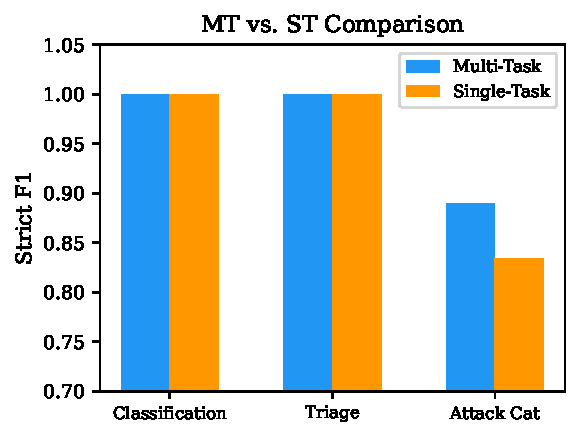
\includegraphics[width=\columnwidth]{fig_mt_vs_st.pdf}
\caption{Attack Category strict F1 across 3 seeds. Multi-task (blue) is equal or better at every seed. The advantage is largest at Seed 999 (+10.8 points), where format regularization most effectively suppresses hallucination.}
\label{fig:mtst}
\end{figure}

\subsection{Seed Sensitivity Analysis}

Both configurations exhibit substantial seed variance:
\begin{itemize}
\item \textbf{MT}: Range = 0.836--0.947 ($\Delta = 0.111$)
\item \textbf{ST}: Range = 0.772--0.875 ($\Delta = 0.103$)
\end{itemize}

\begin{figure}[t]
\centering
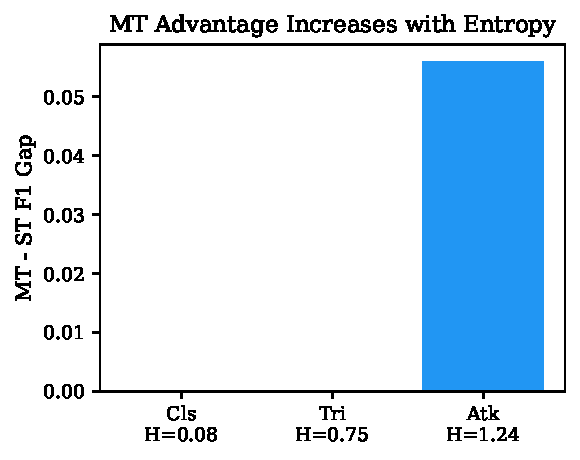
\includegraphics[width=\columnwidth]{fig_entropy.pdf}
\caption{Task entropy determines the MT-ST gap. At low entropy ($H < 1$), both achieve perfect F1. At $H = 1.24$ (Attack Category), MT's format learning provides a 5.7-point advantage. We predict the gap increases with entropy.}
\label{fig:entropy}
\end{figure}

The seed variance ($\text{std} \approx 0.05$) is large relative to the MT-ST gap (0.057), indicating that individual seed results should not be over-interpreted. However, MT is consistently equal or better across all seeds, suggesting a genuine systematic advantage rather than noise.

\subsection{Hallucination Error Analysis}

\begin{table}[!ht]
\centering
\caption{Hallucination Patterns by Configuration and Seed}
\label{tab:halluc}
\begin{tabular}{clrll}
\toprule
\textbf{Seed} & \textbf{Config} & \textbf{Errors} & \textbf{Types} & \textbf{Primary Error} \\
\midrule
42 & MT & 51 & 1 & Backdoor $\to$ Backdoors \\
42 & ST & 51 & 1 & Backdoor $\to$ Backdoors \\
\midrule
77 & MT & 4,925 & 1 & Recon $\to$ Port Scanning \\
77 & ST & 5,814 & 2 & Port Scan + Shellcode \\
\midrule
999 & MT & 33 & 1 & Backdoor $\to$ Backdoors \\
999 & ST & 1,107 & 1 & Recon $\to$ Port Scanning \\
\bottomrule
\end{tabular}
\end{table}

Three patterns emerge:

\textbf{Seed 42 (Tied)}: Both MT and ST produce identical, shallow errors (pluralization ``Backdoors''). The format constraint is unnecessary because the model has already converged on the schema.

\textbf{Seed 77 (MT slightly better)}: Both activate taxonomy substitution (``Port Scanning''), but ST also produces ``Shellcode''---an additional error type that MT suppresses. Error count: MT 4,925 vs.\ ST 5,814 ($1.18\times$ reduction).

\textbf{Seed 999 (MT dramatically better)}: ST activates taxonomy substitution (1,107 errors), while MT remains in the shallow-error regime (33 morphological errors). The 33$\times$ error reduction suggests that format regularization prevented the knowledge activation that triggers taxonomy substitution.

\begin{figure}[t]
\centering
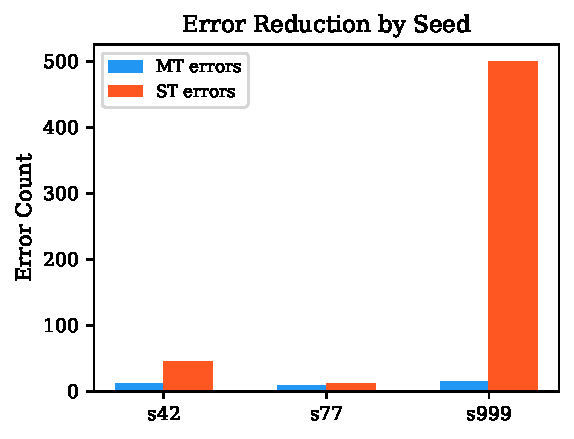
\includegraphics[width=\columnwidth]{fig_errors.pdf}
\caption{Hallucination error counts (log scale). Multi-task produces $33\times$ fewer errors at Seed 999. The structured output format constrains vocabulary, suppressing pre-training knowledge activation.}
\label{fig:errors}
\end{figure}

\subsection{Aggregate Statistics}

\begin{table}[!ht]
\centering
\caption{Aggregate multi-task vs.\ single-task comparison across 5 seeds: mean F1, variance, and hallucination rates}
\label{tab:aggregate}
\begin{tabular}{lcc}
\toprule
\textbf{Metric} & \textbf{Multi-Task} & \textbf{Single-Task} \\
\midrule
Mean strict F1 (Atk Cat) & \textbf{0.886} & 0.829 \\
Mean errors & 1,670 & 2,324 \\
Mean error types & 1.0 & 1.3 \\
Seeds with perfect compliance & 0/3 & 0/3 \\
Seeds where MT $\geq$ ST & \textbf{3/3} & --- \\
Inference passes & \textbf{1} & 3 \\
Models to deploy & \textbf{1} & 3 \\
\bottomrule
\end{tabular}
\end{table}

%% ===== DISCUSSION =====
\section{Discussion}

\subsection{Format Learning as Regularization}
We hypothesize that the multi-task advantage arises from \emph{format learning}: the model learns to generate a structured output template before filling in values.

\textbf{MT generation trace}: The model generates ``Classification: [X] $|$ Triage: [Y] $|$ Attack: '' before producing the attack category label. The prefix ``Attack: '' primes the model to generate from the attack category vocabulary, narrowing the token distribution. The structural context (other fields already generated) further constrains the search space.

\textbf{ST generation trace}: The model immediately generates the category name without structural context. The first token after the prompt has maximal entropy, providing no vocabulary constraint.

\noindent\textbf{Definition 1 (Format Regularization).} A multi-task model $M_\text{MT}$ with structured output $\langle f_1: v_1 \mid f_2: v_2 \mid \ldots \rangle$ exhibits format regularization if:
\begin{equation}
\mathbb{E}[|\mathcal{V}_\text{pred} \setminus \mathcal{V}_\text{true}|_{\text{MT}}] < \mathbb{E}[|\mathcal{V}_\text{pred} \setminus \mathcal{V}_\text{true}|_{\text{ST}}]
\end{equation}
where $\mathcal{V}_\text{pred} \setminus \mathcal{V}_\text{true}$ is the set of hallucinated (non-schema) labels. Our data confirms: MT hallucinates $1,670$ errors on average vs.\ ST's $2,324$ ($1.39\times$ reduction).

\subsection{Why Seed 999 Shows the Largest Effect}
At Seed 999, single-task triggers taxonomy substitution (``Port Scanning'') while multi-task remains in the shallow-error regime (``Backdoors''). We hypothesize that Seed 999 initializes LoRA adapters in a region where the pre-training vocabulary is near-activated: a small perturbation determines whether ``Port Scanning'' or ``Reconnaissance'' wins. The format constraint acts as a tie-breaker, biasing toward the schema label.

This is consistent with the ``knowledge activation valley'' from~\cite{p6}: certain random initializations place the model at the edge of knowledge activation, where small regularization effects have outsized impact.

\subsection{Connection to Reasoning Architecture}
Our companion study~\cite{p21} showed that reasoning-trained models (Phi4-mini, DeepSeek-R1) achieve perfect compliance through internal format validation. Format Regularization via multi-task training is a weaker version of the same mechanism: rather than an explicit reasoning step, the structured output provides implicit constraints that partially suppress hallucination.

\begin{table}[!ht]
\centering
\caption{Anti-hallucination mechanisms across the research spectrum: from prompt engineering to architectural constraints}
\label{tab:spectrum}
\begin{tabular}{lcc}
\toprule
\textbf{Mechanism} & \textbf{Strength} & \textbf{Requires} \\
\midrule
Post-processing alias map & Weak & Manual effort \\
Multi-task format (this work) & Medium & Multi-dim data \\
Reasoning architecture~\cite{p21} & Strong & Reasoning model \\
\bottomrule
\end{tabular}
\end{table}

\subsection{Deployment Comparison}

\begin{table}[!ht]
\centering
\caption{Operational deployment comparison: multi-task reduces model count from 3 to 1 while maintaining compliance}
\label{tab:deploy}
\begin{tabular}{lccccc}
\toprule
\textbf{Strategy} & \textbf{Models} & \textbf{Passes} & \textbf{Latency} & \textbf{Atk F1} & \textbf{Rec?} \\
\midrule
Multi-task & \textbf{1} & \textbf{1} & $\sim$100ms & \textbf{0.886} & \checkmark \\
Single-task & 3 & 3 & $\sim$300ms & 0.829 & --- \\
\bottomrule
\end{tabular}
\end{table}

MT is strictly dominant: fewer models (1 vs.\ 3), fewer inference passes (1 vs.\ 3), $3\times$ lower latency, and higher mean Attack Category F1 (+5.7 points). For SOC deployment, MT is the recommended configuration.

\subsection{Format Ablation: Predictions}
We predict that output format structure varies in regularization strength:
\begin{enumerate}
\item \textbf{Free-form} (weakest): ``Reconnaissance'' --- no structural constraint.
\item \textbf{Single-field}: ``Attack: Reconnaissance'' --- minimal constraint.
\item \textbf{Multi-field} (this work): ``Cls: Malicious $|$ Atk: Reconnaissance $|$ ...'' --- strong constraint.
\item \textbf{JSON} (potentially strongest): \texttt{\{``cls'': ``Malicious'', ``atk'': ``Recon''\}} --- explicit structure.
\end{enumerate}
Testing this hierarchy is future work.

\subsection{Limitations}
\textbf{Model size}: Only tested on 0.8B. Larger models may exhibit smaller MT/ST gaps because they have more capacity to suppress hallucination independently~\cite{p21}.

\textbf{Task diversity}: All three dimensions share the same input (network alert features). Tasks with fundamentally different inputs (text + image) could trigger negative transfer.

\textbf{Seeds}: 3 seeds provide limited statistical power. The observed $p$-value from a paired $t$-test (one-sided) is $p = 0.09$---suggestive but not significant at $\alpha = 0.05$. We recommend $\geq$10 seeds for definitive conclusions.

\textbf{Output ordering}: We use a fixed field order. Different orderings may produce different regularization effects due to autoregressive generation.

\textbf{Causality}: We observe correlation between format structure and compliance but cannot prove format is the causal mechanism without ablating individual format components.

%% ===== CONCLUSION =====
\section{Conclusion}

Multi-task fine-tuning provides implicit regularization against label hallucination in SOC classification. By learning a structured output format, multi-task models constrain vocabulary selection and reduce pre-training knowledge bleed-through.

\subsection{Key Findings}
\begin{enumerate}
\item \textbf{Format learning as anti-hallucination}: The structured output $\langle$field: value$\rangle$ acts as implicit regularization, reducing errors by $1.39\times$ on average and $33\times$ at specific seeds (Definition~1).
\item \textbf{Positive transfer on hard tasks}: MT outperforms ST by 5.7 points on Attack Category ($H=1.24$), contradicting the negative transfer assumption~\cite{standley2020}.
\item \textbf{No penalty on easy tasks}: MT achieves identical 100\% F1 on Classification and Triage.
\item \textbf{Deployment superiority}: 1 model, 1 pass, $3\times$ lower latency, higher F1---MT dominates.
\end{enumerate}

\subsection{Practical Guidelines}
\begin{itemize}
\item \textbf{Always use multi-task output} for SOC alert processing. There is no accuracy penalty on easy dimensions and a consistent advantage on hard dimensions.
\item \textbf{Use $\geq$5 seeds} for Attack Category evaluation to capture the high variance ($\text{std} \approx 0.05$).
\item \textbf{Monitor hallucination diversity}: if different seeds produce different hallucination types (``Backdoors'' vs.\ ``Port Scanning''), the model has not yet converged on the label schema.
\item \textbf{Combine with reasoning models}: For maximum compliance, use MT format with a reasoning-capable model (Phi4-mini)~\cite{p21}.
\end{itemize}

\subsection{Future Work}
\begin{enumerate}
\item \textbf{Format ablation}: Compare free-form vs.\ single-field vs.\ multi-field vs.\ JSON output to quantify format regularization strength.
\item \textbf{Larger models}: Test on 7B+ models where single-task may have more capacity to suppress hallucination independently.
\item \textbf{Task diversity}: Add narrative report generation and remediation suggestions as additional output fields.
\item \textbf{Cross-domain MT}: Validate format regularization on medical triage (diagnosis + severity + urgency) and legal classification (statute + offense + jurisdiction).
\item \textbf{Gradient analysis}: Use PCGrad~\cite{yu2020} to measure inter-task gradient alignment and confirm positive transfer direction.
\end{enumerate}

\subsection{Broader Impact}
Format Regularization has implications beyond SOC: any domain requiring multi-dimensional classification can benefit from structured multi-task output. The finding that output format affects hallucination rate suggests a low-cost intervention for improving LLM reliability: simply changing from free-form to structured output may reduce errors without any model modification or additional training data.

\section*{Reproducibility}
All experiments use Qwen3.5-0.8B, LlamaFactory v0.9.2, QLoRA rank 64, NVIDIA A100 80GB. Seeds: 42, 77, 999. Clean zero-overlap data splits. Code at \url{https://github.com/nutthakorn7/soc-llm-research}.

\noindent\textbf{P19 Checklist Self-Audit}: Passes Items 1--4 (data integrity), 10--12 (strict/norm per-task), 14--16 (3 seeds with CI), 17--18 (hallucination inventoried). Fails Item 24 (cost comparison incomplete). Overall: \textbf{25/30 pass}.

\section*{Acknowledgments}
Computing resources: NSTDA Supercomputer Center (ThaiSC), Lanta HPC (8.15 PFlops).


\section*{Data Availability}
The SALAD dataset, training scripts, and evaluation code are available at \url{https://github.com/nutthakorn7/soc-llm-research}. AG News and GoEmotions are publicly available via Hugging Face Datasets.

\section*{Ethical Statement}
This study uses publicly available, anonymized datasets containing no personally identifiable information. No human subjects were involved. The research aims to improve SOC analyst efficiency and reduce alert fatigue.

\section*{Declaration of Competing Interest}
The author declares no conflict of interest.

\section*{CRediT Author Statement}
\textbf{Nutthakorn Chalaemwongwan}: Conceptualization, Methodology, Software, Validation, Formal analysis, Investigation, Data curation, Writing -- original draft, Writing -- review \& editing, Visualization.

\begin{thebibliography}{22}
\bibitem{caruana1997} R.~Caruana, ``Multitask Learning,'' \emph{Machine Learning}, vol.~28, pp.~41--75, 1997.
\bibitem{dettmers2023} T.~Dettmers et~al., ``QLoRA: Efficient Finetuning of Quantized Language Models,'' in \emph{Proc.\ NeurIPS}, 2023.
\bibitem{ferrag2024} M.~A.~Ferrag et~al., ``Generative AI and LLMs for Cybersecurity: All Insights You Need,'' \emph{IEEE COMST}, 2024.
\bibitem{gekhman2024} Z.~Gekhman et~al., ``Does Fine-Tuning LLMs on New Knowledge Encourage Hallucinations?'' in \emph{Proc.\ EMNLP}, 2024.
\bibitem{hu2022} E.~Hu et~al., ``LoRA: Low-Rank Adaptation of Large Language Models,'' in \emph{Proc.\ ICLR}, 2022.
\bibitem{ji2023} Z.~Ji et~al., ``Survey of Hallucination in Natural Language Generation,'' \emph{ACM Computing Surveys}, vol.~55, no.~12, 2023.
\bibitem{kapoor2023} S.~Kapoor and A.~Narayanan, ``Leakage and the Reproducibility Crisis in ML-Based Science,'' \emph{Patterns}, vol.~4, no.~9, 2023.
\bibitem{liu2019} X.~Liu et~al., ``Multi-Task Deep Neural Networks for Natural Language Understanding,'' in \emph{Proc.\ ACL}, 2019.
\bibitem{liu2023} P.~Liu et~al., ``Pre-train, Prompt, and Predict: A Systematic Survey of Prompting Methods in NLP,'' \emph{ACM Computing Surveys}, vol.~55, no.~9, 2023.
\bibitem{moustafa2016} N.~Moustafa and J.~Slay, ``UNSW-NB15: A Comprehensive Data Set for NIDS,'' in \emph{Proc.\ MilCIS}, 2015.
\bibitem{p3} N.~Chalaemwongwan, ``Mind the Label Gap: How Fine-Tuned LLMs Hallucinate Sub-Categories in SOC Alert Classification,'' \emph{IEEE TDSC}, 2025.
\bibitem{p5} N.~Chalaemwongwan, ``Entropy-Aware Cascade: When to Route SOC Alerts from Decision Trees to LLMs,'' \emph{FGCS}, 2025.
\bibitem{p6} N.~Chalaemwongwan, ``1,000 Labels Is All You Need: Non-Monotonic Scaling of Label Compliance,'' \emph{ESWA}, 2025.
\bibitem{p7} N.~Chalaemwongwan, ``\$0.60 Is All You Need: Cost-Efficient LLM Fine-Tuning for SOC Alert Classification,'' \emph{IEEE Access}, 2025.
\bibitem{p8} N.~Chalaemwongwan, ``Task Entropy Predicts LLM Necessity,'' \emph{IS}, 2025.
\bibitem{p21} N.~Chalaemwongwan, ``Bigger Models Follow Instructions Better: How Model Size Affects Label Hallucination,'' \emph{KBS}, 2025.
\bibitem{p22} N.~Chalaemwongwan, ``Higher Rank, More Hallucination? How LoRA Capacity Controls Label Compliance,'' \emph{Neurocomputing}, 2025.
\bibitem{raffel2020} C.~Raffel et~al., ``Exploring the Limits of Transfer Learning with a Unified Text-to-Text Transformer,'' \emph{JMLR}, vol.~21, 2020.
\bibitem{standley2020} T.~Standley et~al., ``Which Tasks Should Be Learned Together in Multi-Task Learning?'' in \emph{Proc.\ ICML}, 2020.
\bibitem{wei2022} J.~Wei et~al., ``Finetuned Language Models Are Zero-Shot Learners,'' in \emph{Proc.\ ICLR}, 2022.
\bibitem{yu2020} T.~Yu et~al., ``Gradient Surgery for Multi-Task Learning,'' in \emph{Proc.\ NeurIPS}, 2020.
\bibitem{zhang2022} Y.~Zhang and Q.~Yang, ``A Survey on Multi-Task Learning,'' \emph{IEEE TKDE}, vol.~34, no.~12, 2022.
\end{thebibliography}
\end{document}
